\documentclass[a4paper]{article}

\usepackage[UTF8]{ctex}
\usepackage{graphicx}
\usepackage{xurl}
\usepackage{cite}
\usepackage{hyperref}
\usepackage{amsmath}
\hypersetup{
    colorlinks=true,
    allcolors=black,
    breaklinks=true
}

\begin{document}

\songti

\title{电力电子技术基础第二次作业}
\author{2018040401018 李金豪}

\maketitle

\section{Question 2}

Q:使晶闸管导通的条件是什么?

A:晶闸管承受正向电压,且仅在门级有触发电流的情况下才会导通

\section{Question 3}

Q:维持晶闸管导通的条件是什么?怎样才能使晶闸管由导通变为关断?

A:维持导通——流过晶闸管的电流大于维持电流$I_H$ 由导通变为关断——利用外加电压和外电路的作用使流
过晶闸管的电流降到$I_H$以下

\section{Question 4}

Q:阴影部分为晶闸管处于通态区间的电流波形,各波形的电流最大值均为$I_m$,试计算各波形的电流平均值
$I_{d1}$、$I_{d2}$、$I_{d3}$与电流有效值$I_{1}$、$I_{2}$、$I_{3}$

A:

\begin{equation}
    \begin{aligned}
        I_{d1} & = \frac{1}{2\pi}\int_{\frac{\pi}{4}}^{\pi} I_m \sin{\omega t} d(\omega t) \\
               & = \frac{I_m}{2\pi}\times (\frac{\sqrt{2}}{2}+1)                           \\
               & = 0.27I_m
    \end{aligned}
\end{equation}

\begin{equation}
    \begin{aligned}
        I_{d2} & = 2\times\frac{1}{2\pi}\int_{\frac{\pi}{4}}^{\pi} I_m \sin{\omega t} d(\omega t) \\
               & = \frac{I_m}{\pi}(\frac{\sqrt{2}}{2}+1)                                          \\
               & = 0.54I_m
    \end{aligned}
\end{equation}

\begin{equation}
    \begin{aligned}
        I_{d3} = \frac{I_m\times \frac{\pi}{2}}{2\pi} = 0.25I_m
    \end{aligned}
\end{equation}

\begin{equation}
    \begin{aligned}
        I_1 = \sqrt{\frac{1}{2\pi} \int_{\frac{\pi}{4}}^{\pi} (I_m\sin\omega t)^2 d(\omega t)} = 0.48I_m
    \end{aligned}
\end{equation}

\begin{equation}
    \begin{aligned}
        I_2 = \sqrt{2\times \frac{1}{2\pi} \int_{\frac{\pi}{4}}^{\pi} (I_m\sin\omega t)^2 d(\omega t)} = 0.67I_m
    \end{aligned}
\end{equation}

\begin{equation}
    \begin{aligned}
        I_3 = \sqrt{\frac{1}{2\pi} \int_{0}^{\frac{\pi}{2}} (I_m)^2 d(\omega t)} = 0.5I_m
    \end{aligned}
\end{equation}

\section{Question 5}

Q:上题若不考虑安全裕量,问100A的晶闸管能送出平均电流$I_{d1}$、$I_{d2}$、$I_{d3}$分别为多少?
这时,相应的电流最大值$I_{m1}$、$I_{m2}$、$I_{m3}$分别为多少?

A:已知晶闸管的通态平均电流$I_{T(AV)}=100A$,可得流过晶闸管电流的有效值为

\begin{equation}
    I_{RMS} = 1.57\times I_{T(AV)} = 157A
\end{equation}

在上题中 $I_1 = 0.48I_{m1}$、$I_2 = 0.67I_{m2}$、$I_3 = 0.5I_{m3}$

\begin{equation}
    \begin{aligned}
        I_{m1} & = \frac{I_{1RMS}}{0.48}=327.08A \\
        I_{m2} & = \frac{I_{2RMS}}{0.67}=234.33A \\
        I_{m3} & = \frac{I_{3RMS}}{0.5}=314.00A
    \end{aligned}
\end{equation}

再根据电流最大值和平均值的关系得

\begin{equation}
    \begin{aligned}
        I_{d1} & = 0.27\times I_{m1} = 88.31A  \\
        I_{d2} & = 0.54\times I_{m2} = 126.54A \\
        I_{d3} & = 0.25\times I_{m3} = 78.50A
    \end{aligned}
\end{equation}

\section{Question 8}

Q:试分析IGBT和电力MOSFET在内部结构和开关特性上的相似与不同之处

A:内部结构——IGBT比VDMOSFET多了一层$P^{+}$注入区,形成了一个大面积的$P^{+}N$结$J_1$,使得IGBT导通时
注入区向漂移区发射少子,实现对漂移区电导率的调制,使得IGBT具有很强的通流能力

开关特性——因为IGBT是双极型器件,在导通时会发生电导调制效应,导通损耗比MOSFET小;但正由于
IGBT是少子器件,会有少子储存,关断时间慢于MOSFET,会有拖尾电流

\section{Question 9}

Q:试列举典型的宽禁带半导体材料。基于这些宽禁带半导体材料的电力电子器件在哪些方面性能优于硅器件?

A:典型宽禁带半导体——碳化硅、氮化镓、金刚石

具有比硅器件高得多的耐受高电压能力、低得多的通态电阻、更好的导热性能和热稳定性
以及更强的耐受高温和射线辐射的能力,许多方面的性能都是成数量级的提高

\section{Question}

Q:电感的电流波形和电容的电压波形

A:开关闭合后,根据基尔霍夫电压定律有

\begin{equation}
    \begin{aligned}
         & L\frac{di(t)}{dt}+u_c(t)+i(t)R=300                                                        \\
         & \Rightarrow LC\frac{d^2}{dt^2}u_c(t)+RC\frac{du_c(t)}{dt}+u_c(t) = 300                    \\
         & \Rightarrow \frac{d^2}{dt^2}u_c(t)+1\times 10^{(-6)}\times \frac{du_c(t)}{dt} +u_c(t) = 300
    \end{aligned}
\end{equation}

该二阶非齐次常微分方程的解由其对应的齐次方程的通解和非齐次的特解组成。先求解对应的
齐次方程的通解

\begin{equation}
    \begin{aligned}
        \frac{d^2}{dt^2}u_c(t)+1\times 10^{(-6)}\times\frac{du_c(t)}{dt}+u_c(t) = 0
    \end{aligned}
\end{equation}

上式对应的特征方程为

\begin{equation}
    \begin{aligned}
        \lambda^2+1\times 10^{(-6)}\lambda+1=0
    \end{aligned}
\end{equation}

解得特征根为

\begin{equation}
    \begin{aligned}
        \lambda_1 = -\frac{R}{2L}+\frac{\sqrt{(RC)^2-4LC}}{2LC} &= (-0.5+j0.87)\times 10^{6}\\
        \lambda_2 = -\frac{R}{2L}-\frac{\sqrt{(RC)^2-4LC}}{2LC} &= (-0.5-j0.87)\times 10^{6}
    \end{aligned}
\end{equation}

故该齐次方程的通解为

\begin{equation}
    \begin{aligned}
        u_{cc}(t) = \exp(-0.5\times 10^{6}t)\times (C_1\cos0.87\times 10^6 t+C_2\sin0.87\times 10^6 t)
    \end{aligned}
\end{equation}

由于电压源为直流,故非齐次微分方程的特解为

\begin{equation}
    \begin{aligned}
        u_{cs}(t) = 300
    \end{aligned}
\end{equation}

综上,该非齐次常微分方程的通解为

\begin{equation}
    \begin{aligned}
        u_{c}(t) = \exp(-0.5\times 10^{6}t)\times (C_1\cos0.87\times 10^6 t+C_2\sin0.87\times 10^6 t) + 300
    \end{aligned}
\end{equation}

最后根据初值条件求解$C_1$和$C_2$的值

\begin{equation}
    \begin{cases}
        &u_c(0) = C_1+300=0\\
        &\frac{du_c(t)}{dt}\mid_{t=0} = 0
    \end{cases}
\end{equation}

解得

\begin{equation}
    \begin{cases}
        &C_1 = -300\\
        &C_2 = -172.4
    \end{cases}
\end{equation}

故电容电压的表达式为

\begin{equation}
    u_{c}(t) = \exp(-0.5\times 10^{6}t)\times (-300\cos0.87\times 10^6 t-172.4\sin0.87\times 10^6 t) + 300 \quad (V)
\end{equation}

由$i(t) = C\frac{du_c(t)}{dt}$解得电感电流表达式

\begin{equation}
    i(t) = \exp(-0.5\times 10^{6}t)\times(34.72\sin0.87\times 10^6t-1.2\times 10^(-3)\cos0.87\times 10^6t)  \quad (A)
\end{equation}

用Matlab画出电感电流和电容电压波形如下

\begin{figure}[htbp]
    \centering
    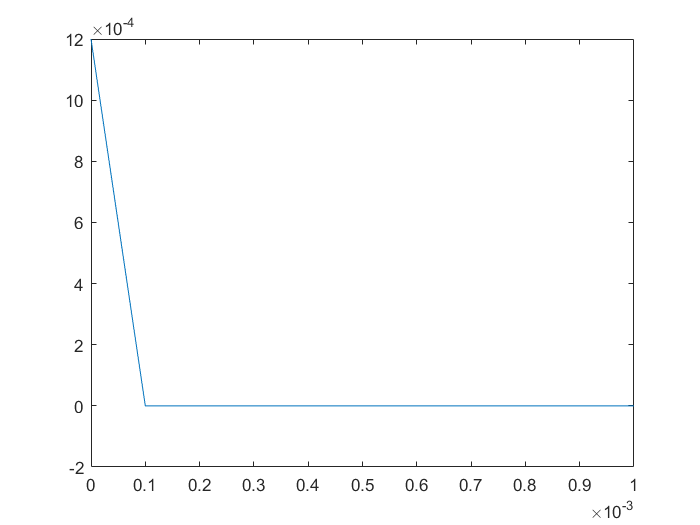
\includegraphics[width=12cm,height=6cm]{current2.PNG}
    \caption{电感电流波形}
\end{figure}

\begin{figure}[htbp]
    \centering
    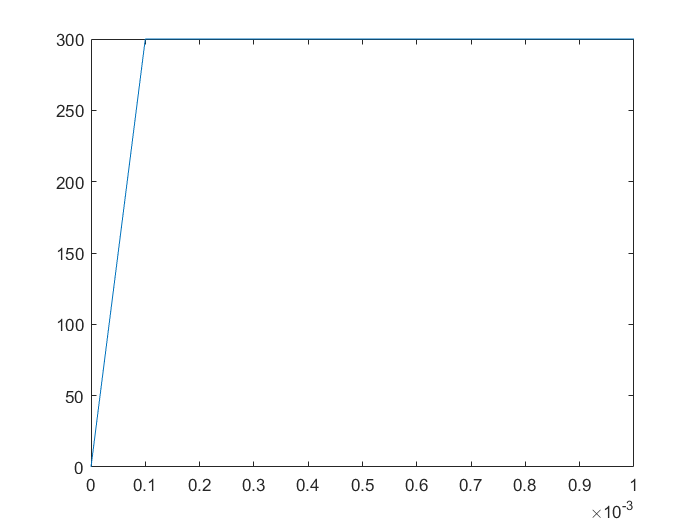
\includegraphics[width=12cm,height=6cm]{voltage2.PNG}
    \caption{电容电压波形}
\end{figure}

\end{document}